\documentclass[11pt,a4paper]{article}
\usepackage[margin=2.4cm]{geometry}
\usepackage{fontspec}
\usepackage{unicode-math}
\setmainfont{STIX Two Text}
\setmathfont{STIX Two Math}
\directlua{luaotfload.add_fallback("leanfb", {"STIX Two Math:mode=harf;", "STIXGeneral:mode=harf;"})}
\setmonofont{Menlo}[Scale=0.80,RawFeature={fallback=leanfb}]
\usepackage{fancyvrb}
\usepackage{xcolor}
\usepackage{booktabs}
\usepackage{tabularx}
\usepackage{enumitem}
\usepackage{tikz}
\usetikzlibrary{arrows.meta,positioning,cd}
\usepackage[colorlinks=true,linkcolor=blue!50!black,urlcolor=blue!50!black]{hyperref}

\definecolor{codebg}{gray}{0.96}
\DefineVerbatimEnvironment{lean}{Verbatim}{fontsize=\footnotesize,frame=single,rulecolor=\color{gray!50},framesep=2mm,commandchars=§«»}
\newcommand{\lsub}[1]{\textsubscript{#1}}
\newcommand{\code}[1]{\texttt{#1}}
\newcommand{\cA}{\mathcal{A}}
\newcommand{\Ocal}{\mathcal{O}}
\newcommand{\dbar}{\bar\partial}
\newcommand{\Ho}{\mathrm{Ho}}
\newcommand{\Dperf}{D_{\mathrm{perf}}}
\newcommand{\Hom}{\mathrm{Hom}}
\newcommand{\X}{\mathbb{X}}
\newcommand{\hc}{\check h}
\setlist{itemsep=2pt,topsep=4pt}
\emergencystretch=4em

\title{Block's theorem in Lean 4\\[4pt]
\large Summary of the formalization: the statements and the proof strategy}
\author{Project \code{cohesivemodules} (Lean 4 + Mathlib \code{v4.35.0})}
\date{9 November 2026}

\begin{document}
\maketitle

\begin{abstract}
We summarize a Lean 4 formalization of J.~Block's comparison theorem between cohesive modules
over the Dolbeault algebra and perfect complexes, in the form proved by P.~Antweiler. For every
compact Hausdorff complex manifold $X$, the functor
$J\colon \Ho(\mathcal P_A)\to D(\Ocal_X)$, $M\mapsto\alpha(M)$, is fully faithful with essential
image exactly $\Dperf(X,\Ocal_X)$. The Lean theorem \code{main\_theorem : MainStatement} is proved
without \code{sorry} and without further hypotheses; it depends only on the axioms
\code{propext}, \code{Classical.choice}, \code{Quot.sound}. The two analytic inputs, the
Dolbeault--Grothendieck lemma (H1) and a weak local gauge lemma (H2), are proved in the project.
We also prove the twisted form (\cite[Thm~7.4.3]{A}): for a $\dbar$-closed $h\in\cA^{0,2}(X)$, cohesive
modules over the curved algebra $(\cA_X(X),\dbar,h)$ are equivalent to perfect complexes of
$\hc$-twisted $\Ocal_X$-modules. We explain the Lean statements and the definitions they rest on,
then the proofs, layer by layer, with the places where the formal proof deviates from the
sources.
\end{abstract}

\tableofcontents

%======================================================================
\section{The theorem}

\paragraph{Sources.} Block \cite[Thm~4.1.3]{B}; Antweiler \cite[Thm~7.2.20 and Thm~7.4.3]{A};
\cite{CHL} for the comparison theorem in the abstract setting. For the analytic lemmas:
\cite{Hor, GH, DK, BSW}; for twisted sheaves: \cite{Cal, Toda}; for the triangulated structure:
\cite{BK}. The formalization is built on Mathlib \cite{Mathlib}.

\paragraph{Informal statement.} Let $E$ be a finite-dimensional complex normed space and $X$ a
compact Hausdorff complex manifold modelled on $E$. Let $A=\cA_X(X)=\cA^{0,\bullet}(X)$ be the
Dolbeault algebra of $X$ (smooth $(0,q)$-forms with $\dbar$ and wedge product) and $\Ocal_X$ the
sheaf of holomorphic functions. Then the functor
\[ J\colon \Ho(\mathcal P_A)\longrightarrow D(\Ocal_X),\qquad M\longmapsto \alpha(M), \]
from the homotopy category of cohesive modules over $A$ to the derived category of sheaves of
$\Ocal_X$-modules, is full and faithful, and its essential image is $\Dperf(X,\Ocal_X)$. In other
words, $J$ corestricts to an equivalence $\Ho(\mathcal P_A)\simeq\Dperf(X)$.

\paragraph{History of the statement.} The project first proved the theorem under two analytic
hypotheses on $X$:
\begin{itemize}
\item[(H1)] \emph{Dolbeault--Grothendieck lemma}: $\dbar$-closed $(0,q{+}1)$-forms are locally
$\dbar$-exact;
\item[(H2)] \emph{local gauge lemma, weak form}: every cohesive module over $A$ is, near each
point, homotopy equivalent to one coming from a bounded complex of finitely generated projective
$\Ocal$-modules.
\end{itemize}
Both are true on every complex manifold (H1 is classical; H2 is the content of the proof of
\cite[Lemma~4.1.5]{B}), and both are now theorems of the project (\S\ref{sec:h1}, \S\ref{sec:h2}). The
conditional statement is kept, as a corollary, under the name \code{MainStatementConditional}.

\subsection{The Lean statement}
The statement lives in \code{Cohesivemodules/Statements.lean}, which imports only files marked
\code{-- FROZEN} (definitions checked in excerpts at a review gate, which may not be changed)
and Mathlib:
\begin{lean}
def MainStatement : Prop :=
  ∀ (E : Type) [NormedAddCommGroup E] [NormedSpace ℂ E] [FiniteDimensional ℂ E]
    (X : Type) [TopologicalSpace X] [T2Space X] [CompactSpace X]
    [ChartedSpace E X] [IsManifold 𝓘(ℂ, E) ∞ X],
      letI := HasDerivedCategory.standard (Mod (ringOf (holSheaf E X)))
      (blockFunctor E X).Full ∧ (blockFunctor E X).Faithful ∧
        (blockFunctor E X).essImage = Perf (ringOf (holSheaf E X))
\end{lean}
and the theorem, in \code{MainH2.lean}:
\begin{lean}
theorem main_theorem : Cohesive.MainStatement
-- #print axioms main_theorem : [propext, Classical.choice, Quot.sound]
\end{lean}
Reading the statement line by line:
\begin{itemize}
\item \code{IsManifold 𝓘(ℂ, E) ∞ X}: $X$ has an atlas with complex-$C^\infty$ (that is,
holomorphic) transition maps. In Mathlib $\infty$ means $C^\infty$; $\top$ would mean
analytic ($C^\omega$). We checked the elaborated statement: the exponent is $\infty$.
\item \code{T2Space X}, \code{CompactSpace X}: compact Hausdorff; these are implicit in the
sources.
\item \code{blockFunctor E X : HoP (dolbeault E X) ⥤ DerivedCategory (Mod (ringOf (holSheaf E X)))}:
the functor $J$ (\S\ref{sec:J}).
\item \code{Perf R}: the objects of $D(R)$ isomorphic to $Q(K)$ for a perfect complex $K$
(\S\ref{sec:perf}).
\item \code{HasDerivedCategory.standard}: Mathlib's derived category is defined relative to an
instance (a choice of universe and of localization); the statement fixes the standard one,
once, for both \code{blockFunctor} and \code{Perf}.
\end{itemize}
The conditional form \code{MainStatementConditional} (\code{StatementsConditional.lean}, frozen
at gate~5) is the same statement with the premises
\code{DolbeaultGrothendieck E X → LocalGaugeLemma E X →} after the binders; it is proved in
\code{Main.lean} as \code{main\_theorem\_conditional}, and \code{main\_theorem} applies it to the
proofs \code{dolbeaultGrothendieck E X} and \code{localGaugeLemma E X}. (Until 6 November 2026
the conditional statement was called \code{MainStatement} and the present one
\code{MainStatementUnconditional}; the contents did not change.)

\paragraph{Why ``full, faithful, essential image'' and not ``an equivalence onto $\Dperf$''.}
To write a functor $\Ho(\mathcal P_A)\to\Dperf(X)$ one must already know that $\alpha(M)$ is
perfect, which uses H2 (step C2 below). The functor $J$ is therefore defined into the whole
derived category, without using H1 or H2. The check file \code{ChecksMain.lean} proves (K6)
that, for any functor $F$ and any isomorphism-closed property $P$,
\[ F \text{ full} \wedge F\text{ faithful}\wedge \operatorname{essImage}F=P \iff
\exists\, h\colon \forall X,\, P(F X),\ \ (P.\mathrm{lift}\,F\,h) \text{ is an equivalence,} \]
and applies it to \code{blockFunctor} and \code{Perf} (\code{Checks.blockFunctor\_iff}): the
statement is equivalent to ``$J$ corestricts to an equivalence $\Ho(\mathcal P_A)\simeq\Dperf(X)$''.

\paragraph{Sanity checks on the statement.} In complex dimension $0$
($E=\mathrm{Fin}\,0\to\mathbb C$) H1 and H2 are proved directly (K1), independently of their
general proofs, and the point is an example of the theorem (\code{blockPerf\_dim\_zero}).
Non-vacuity of every definition (cohesive modules exist, the Dolbeault data satisfy all fields of
the abstract structures, $\dbar\bar z=d\bar z$ on $\mathbb C$, $\dbar\dbar=0$ and Leibniz on
explicit forms on $\mathbb C^2$) is checked in \code{Checks*.lean}. Further checks of the
definitions behind the statement: $\Hom_{\Ho(\mathcal P_A)}(\cA,\cA[n])\cong H^{0,n}_{\dbar}(X)$
(K4, \S\ref{sec:tr}), and agreement of our $\dbar$ with an independent definition by type
projections (K7, \S\ref{sec:k7}).

\subsection{The twisted theorem}\label{sec:tw-statement}
For a $\dbar$-closed $h\in\cA^{0,2}(X)$, cohesive modules over the \emph{curved} algebra
$(\cA_X(X),\dbar,h)$ have $\X\circ\X=h\cdot(-)$, so $\alpha(M)$ is no longer a complex. On the
members $U_\alpha$ of a finite cover with $h|_{U_\alpha}=\dbar h^0_\alpha$ the operator
$\X-h^0_\alpha$ is flat, and the local complexes glue by units $u_{\alpha\beta}$ up to a Čech
2-cocycle $\hc$ of units of $\Ocal_X$. \cite[Thm~7.4.3]{A} (stated without proof in \cite[Thm~4.2.1]{B})
says that this identifies $\Ho(\mathcal P_{(A,\dbar,h)})$ with twisted perfect complexes.
\begin{lean}
def MainStatementTwisted : Prop :=
  ∀ (E : Type) [NormedAddCommGroup E] [NormedSpace ℂ E] [FiniteDimensional ℂ E]
    (X : Type) [TopologicalSpace X] [T2Space X] [CompactSpace X]
    [ChartedSpace E X] [IsManifold 𝓘(ℂ, E) ∞ X]
    (h : DolbeaultClosed2 E X) (T : TwistData E X h),
      letI := HasDerivedCategory.standard (TwMod (dolbeaultPreData E X).toSheafData.O T.U T.ch)
      (twistedBlockFunctor h T).Full ∧ (twistedBlockFunctor h T).Faithful ∧
        (twistedBlockFunctor h T).essImage = TwPerf (dolbeaultPreData E X).toSheafData.O T.U T.ch
\end{lean}
proved in \code{MainTwisted.lean} as \code{main\_theorem\_twisted}, with the same three axioms.
Here \code{T} is a \emph{twist datum} for $h$ (\S\ref{sec:tw-defs}); one exists for every $h$
(\code{exists\_twistData}), so the statement is not vacuous. The check K8
(\code{K8\_twisted\_implies\_unconditional}) proves \code{MainStatementTwisted → MainStatement}:
at $h=0$ the curved algebra is the flat one by \code{rfl}.

%======================================================================
\section{The definitions behind the statements}
The script \code{scripts/statement\_defs.py} computes, from the compiled environment, every
project declaration that the statements depend on (types and bodies of definitions; proofs are
not followed since they cannot change the meaning). For \code{MainStatement} and
\code{MainStatementConditional} the result is 202 declarations in 25 files, frozen at gates 1--5;
with \code{MainStatementTwisted} it is 276 declarations in 44 files, all frozen at human review gates,
where they were checked in excerpts (the twisted ones at gate~12). Instances on reached types that are not term dependencies (for
example the triangulated structure on \code{HoP}) are listed for information and are not frozen.
This section describes the definitions.

\subsection{Graded-commutative curved dgas (A1)}
A dga is encoded as a $k$-algebra $A$ with a Mathlib \code{GradedAlgebra} structure
$\mathcal A\colon\mathbb Z\to\mathrm{Submodule}\,k\,A$ (internal grading) and a class
\code{GCDga 𝒜} bundling: $\cA^q=0$ for $q<0$ and $q>N$, graded commutativity
$ab=(-1)^{pq}ba$, a degree-one derivation $d$ with graded Leibniz rule and $d^2=0$, and a
curvature $c\in\cA^2$ with $dc=0$ ($d^2=[c,-]$ is automatic, since $c$ is central by graded
commutativity). For Block's theorem $c=0$;
the twisted theorem uses $c=h$. $\cA^0$ is a commutative ring, and $A$ is an $\cA^0$-algebra.

\subsection{Cohesive modules and their homotopy category (A3--A5)}
We use \emph{left} modules (Block uses right modules; the translation is the sign convention
$c\leftrightarrow -c$, and a sanity item A13 proves the two definitions dg-equivalent).
\begin{lean}
structure QuasiCohesive where
  Q : ℤ → Type                         -- generators Q^p, each an 𝒜⁰-module
  X : Tot 𝒜 Q →§lsub«l»[k] Tot 𝒜 Q          -- 𝕏 on the total module A ⊗_{A⁰} ⨁ Q^p
  X_mem   : ...                        -- 𝕏 has total degree 1
  leibniz : ∀ {p} {a}, a ∈ 𝒜 p → ∀ x,
    X (a • x) = GCDga.d a • x + p.negOnePow • a • X x
  flat    : ∀ x, X (X x) = GCDga.c • x

structure CohesiveModule extends QuasiCohesive 𝒜 where
  bounded    : ∃ a b, ∀ p, (p < a ∨ b < p) → Subsingleton (Q p)
  finite     : ∀ p, Module.Finite (𝒜 0) (Q p)
  projective : ∀ p, Module.Projective (𝒜 0) (Q p)
\end{lean}
A cohesive module is thus a bounded graded finitely generated projective $\cA^0$-module $Q$ with a
$\mathbb Z$-graded superconnection $\X$ on $A\otimes_{\cA^0}Q$ with $\X^2=c$ \cite[Def~2.3.2]{B}.

\emph{Hom complexes} (A4): $\Hom^n(M_1,M_2)$ consists of $k$-linear maps $\varphi$ of degree $n$
with $\varphi(a\cdot m)=(-1)^{n|a|}a\cdot\varphi(m)$, and
$\delta\varphi=\X_2\varphi-(-1)^n\varphi\X_1$. The sign convention agrees with Mathlib's
\code{CochainComplex.HomComplex.δ} (proved). \emph{The homotopy category} \code{HoP 𝒜} (A5)
has cohesive modules as objects and $H^0(\Hom^\bullet(M_1,M_2))$ as morphisms (closed degree-0
maps modulo coboundaries).

\emph{Base change} (A9): for a dga map $f\colon A\to B$, $f^*M$ has generators
$B^0\otimes_{A^0}Q^p$ and $\X_B(b\otimes m)=db\otimes m+(-1)^{|b|}b\cdot\X m$; it is used to
restrict cohesive modules to open sets. \emph{Modules from complexes} (A10): for $\rho\colon R\to
A^0$ with $d\rho=0$ and a bounded complex $W$ of finitely generated projective $R$-modules,
$A\otimes_R W$ with $\X=d\otimes1+1\otimes d_W$ (Koszul sign) is cohesive
(\code{CohesiveModule.fromComplex}).

\subsection{\texorpdfstring{Sheaves, perfect complexes, $\Dperf$ (S1, S9)}{Sheaves, perfect complexes, D\_perf (S1, S9)}}\label{sec:perf}
Sheaves of modules are Mathlib's \code{SheafOfModules} over a sheaf of rings
$R$ on \code{Opens X}; \code{Mod R} abbreviates the category. \code{ringOf} turns a sheaf of
commutative rings into a sheaf of rings. Restriction to an open $U$ uses Mathlib's over-site
\code{Over U}.
\begin{lean}
def IsStrictlyPerfect (P : CochainComplex (Mod R) ℤ) : Prop :=
  (∃ a b : ℤ, P.IsStrictlyGE a ∧ P.IsStrictlyLE b) ∧ ∀ n, IsFinFreeSummand (P.X n)

def IsPerfect (K : CochainComplex (Mod R) ℤ) : Prop :=
  ∀ x : X, ∃ U : Opens X, x ∈ U ∧
    ∃ (L P : CochainComplex (Mod (R.over U)) ℤ) (f : L ⟶ K|U) (g : L ⟶ P),
      QuasiIso f ∧ QuasiIso g ∧ IsStrictlyPerfect P

def Perf (R : RingSheaf X) [HasDerivedCategory.{w} (Mod R)] :
    ObjectProperty (DerivedCategory (Mod R)) :=
  fun D ↦ ∃ K, IsPerfect K ∧ Nonempty (D ≅ DerivedCategory.Q.obj K)
\end{lean}
A perfect complex is locally connected by a roof of quasi-isomorphisms to a bounded complex of
direct summands of finite free modules. This is equivalent to the usual
``$Q(K|_U)\cong Q(P)$ in $D(R|_U)$'' but avoids a derived category for every open set.
A sheaf of rings $S$ is \emph{fine} (\code{IsFine}) if every finite open cover admits a partition
of unity $\sum\rho_i=1$ by global sections with $\rho_i$ supported in $U_i$ (in a stalk-free
form). On a compact space finite covers suffice.

\subsection{The Dolbeault algebra and holomorphic functions (F1--F12)}
\begin{itemize}
\item \emph{Fibres} (F2): $\Lambda^{0,q}(E;F)$ is the space of continuous $\mathbb C$-alternating
$q$-linear maps on the conjugate space $\bar E$ (\code{Conj E}, a type synonym with the conjugate
action). A $\mathbb C$-linear map on $\bar E$ is an antilinear map on $E$, so these are exactly
the $(0,q)$-covectors.
\item \emph{$\dbar$ on open subsets of $E$} (F3): $D''\omega(x)=\tfrac12(D\omega(x)+i\,D\omega(x)\circ J)$,
the antilinear part of the real derivative, and $\dbar\omega(x)$ is its alternation (Mathlib's
\code{alternatizeUncurryFin}). $\dbar\dbar=0$ (F4) by copying Mathlib's proof of $d\circ d=0$
with $D''$ for $D$.
\item \emph{Product} (F5): the total fibre $\Lambda^{0,\bullet}=\prod_{q\le n}\Lambda^{0,q}$ gets
its algebra structure transported from Mathlib's exterior algebra of $\mathrm{Dual}_{\mathbb C}\bar
E$ (associativity and graded commutativity for free); Leibniz for $\dbar$ (F6).
\item \emph{Holomorphic pullback} (F7) commutes with $\dbar$; this makes the chart-wise definition
independent of charts.
\item \emph{Sheaves on $X$} (F9--F10): a section of $\cA_X$ over $U$ is a function into the total
fibre, read in charts, whose chart expressions are smooth (a Mathlib \code{LocalPredicate}).
$\cA_X(U)$ is a bounded graded-commutative dga with $\dbar$ (\code{dolbeaultGrade E U}); the
Dolbeault algebra is \code{dolbeault E X := dolbeaultGrade E ⊤}. The degree-$q$ component sheaves
are subtypes of the total section algebra, so that $\cA^0$ is literally the dga's degree-0 part.
\item \emph{Holomorphic functions} (F12): \code{holSheaf E X := smoothSheafCommRing 𝓘(ℂ, E) 𝓘(ℂ, ℂ) X ℂ},
complex-$C^\infty$ functions, which are the holomorphic ones; $\rho\colon\Ocal_X\to\cA^0$ is the
inclusion.
\end{itemize}

\subsection{The hypotheses H1 and H2}\label{sec:hyp}
They are \code{Prop}-valued definitions in \code{Hypotheses.lean} (frozen at gate~3). They occur
in \code{MainStatementConditional} and, as fields, in the abstract resolving data below; they do
not occur in \code{MainStatement}.
\begin{lean}
def DolbeaultGrothendieck : Prop :=
  ∀ (U : Opens X) (q : ℕ) (x : X), x ∈ U →
    ∀ α ∈ dolbeaultGrade E U ((q : ℤ) + 1), GCDga.d α = 0 →
      ∃ (U' : Opens X) (h : U' ≤ U), x ∈ U' ∧
        ∃ η ∈ dolbeaultGrade E U' (q : ℤ), GCDga.d η = (dolbeaultRes E h) α

def LocalGaugeLemma : Prop :=
  ∀ (M : CohesiveModule (dolbeault E X)) (x : X),
    ∃ (U' : Opens X) (_ : x ∈ U')
      (W : CochainComplex (ModuleCat (O_X(U'))) ℤ) (hW : IsBoundedFGProj _ W),
      Nonempty (HoP.mk (M.baseChange (dolbeaultRes E (le_top : U' ≤ ⊤))) ≅
                HoP.mk (CohesiveModule.fromComplex (ρ := dolbeaultRhoU E U') W ...))
\end{lean}
H1 together with F12 says exactly that $0\to\Ocal_X\to\cA^{0,0}\xrightarrow{\dbar}\cA^{0,1}\to\cdots$ is
a resolution. H2 says: near each point, the restriction $M|_{U'}$ is isomorphic in
$\Ho(\mathcal P_{\cA(U')})$ to $\cA(U')\otimes_{\Ocal(U')}W$. It is stated for sections over
small opens, only for restrictions of global modules, which is all the proof uses (\cite{A}'s
Assumption~6 is a sheaf version on every open).

\subsection{\texorpdfstring{The functor $J$ (C0, C1)}{The functor J (C0, C1)}}\label{sec:J}
The comparison is proved for abstract \emph{resolving data}, then applied to the Dolbeault data.
\code{PreResolvingData X} bundles, for a topological space $X$: a presheaf of bounded
graded-commutative dgas $U\mapsto\cA(U)$ that is a sheaf (gluing, locality of degree), with flat
curvature; a sheaf of commutative rings $\Ocal$ and ring maps $\rho_U\colon\Ocal(U)\to\cA^0(U)$,
natural, with $d\circ\rho=0$; $\cA^0$ fine; each $\cA^q$ locally free over $\cA^0$ (local frames).
\code{ResolvingData} adds the resolution condition ($\rho$ injective, exactness in degree $0$ and
in degrees $q+1$) and the local lifting field \code{LL} (the abstract form of H2).

For pre-resolving data $P$ and a cohesive module $M$ over $A=\cA(X)$, the complex
$\alpha(M)$ (Lean: \code{P.sheafOf M}) has
\[ \alpha(M)^n(V) = \bigl(\cA(V)\otimes_{\cA^0(V)}\textstyle\bigoplus_p \cA^0(V)\otimes_{\cA^0(X)}Q^p\bigr)^n
\;\cong\; \textstyle\bigoplus_{p+q=n}\cA^q(V)\otimes_{\cA^0(X)}Q^p, \]
the degree-$n$ part of the total module of the base change $M|_V$, with the differential $\X$ of
$M|_V$; $\Ocal$ acts through $\rho_V$; restriction maps are the base-change maps. (The first form
reuses the base change A9 and its functoriality; it is canonically isomorphic to Block's
formula.) It is a sheaf (C1.a: $Q^p$ is finitely generated projective and $\cA^q$ is a summand of
a finite free $\cA^0$-module). A closed degree-0 map gives a chain map, a coboundary a
null-homotopic one (C1.b), so
\[ J := (\Ho(\mathcal P_A)\to K(\mathrm{Mod}\,\Ocal)\to D(\mathrm{Mod}\,\Ocal)),\qquad
\code{P.J := P.JK ⋙ DerivedCategory.Qh}. \]
Finally (\code{BlockFunctorDef.lean}):
\begin{lean}
def dolbeaultPreData : PreResolvingData X   -- the Dolbeault data; every field a theorem
def blockFunctor [h : HasDerivedCategory.{w} (Mod (ringOf (holSheaf E X)))] :
    HoP (dolbeault E X) ⥤ DerivedCategory (Mod (ringOf (holSheaf E X))) :=
  @PreResolvingData.J X _ (dolbeaultPreData E X) h
\end{lean}
Every field of \code{dolbeaultPreData} is a theorem of layer F: gluing and locality of forms,
$\rho$ natural with $\dbar\rho=0$, $\cA^0$ fine (smooth partitions of unity, needs compact
Hausdorff), $\cA^{0,q}$ locally free of rank $\binom nq$. No analytic hypothesis is used:
\code{blockFunctor} is defined without H1, H2.

\subsection{Curved Dolbeault algebras, twist data, twisted sheaves (Z3)}\label{sec:tw-defs}
\begin{itemize}
\item \code{DolbeaultClosed2 E X}: global forms $h$ of degree $2$ with $\dbar h=0$;
\code{curvedDolbeault h} is $(\cA_X(X),\dbar,h)$, the Dolbeault algebra with curvature replaced
by $h$ (\code{GCDga.withC}, on the same carrier).
\item \code{TwistData E X h}: a finite open cover $U=(U_\alpha)$, primitives
$h^0_\alpha\in\cA^{0,1}(U_\alpha)$ with $\dbar h^0_\alpha=h|_{U_\alpha}$, units
$u_{\alpha\beta}\in\cA^0(U_\alpha\cap U_\beta)^\times$ with
$\dbar u_{\alpha\beta}=(h^0_\beta-h^0_\alpha)u_{\alpha\beta}$, $u_{\alpha\alpha}=1$,
$u_{\beta\alpha}=u_{\alpha\beta}^{-1}$, and a normalized Čech 2-cocycle $\hc$ of units of
$\Ocal_X$ with $\rho(\hc_{\alpha\beta\gamma})=u_{\beta\gamma}u_{\alpha\beta}u_{\alpha\gamma}^{-1}$.
\item \code{TwMod O U ȟ}: $\hc$-twisted sheaves of modules, i.e.\ sheaves $M_\alpha$ on the
over-sites \code{Over U\lsub{α}} with gluing maps $\varphi_{\alpha\beta}$ on sections over every
$W\le U_\alpha\cap U_\beta$, $\varphi_{\alpha\alpha}=\mathrm{id}$ and
$\varphi_{\beta\gamma}\circ\varphi_{\alpha\beta}=\hc_{\alpha\beta\gamma}\varphi_{\alpha\gamma}$. It is an
abelian category (its \code{Abelian} instance is frozen, since the derived category depends on it)
with enough injectives.
\item \code{TwPerf}: objects of $D(\mathrm{TwMod})$ isomorphic to $Q(K)$ with every component
$K_\alpha$ perfect on $U_\alpha$.
\item \code{twistedBlockFunctor h T}: $M$ goes to the twisted complex with components
$\alpha(M)^n|_{U_\alpha}$, differential $\X-h^0_\alpha$ and gluing $u_{\alpha\beta}\cdot$.
\end{itemize}

%======================================================================
\section{The proof}
\subsection{Architecture}
\begin{center}
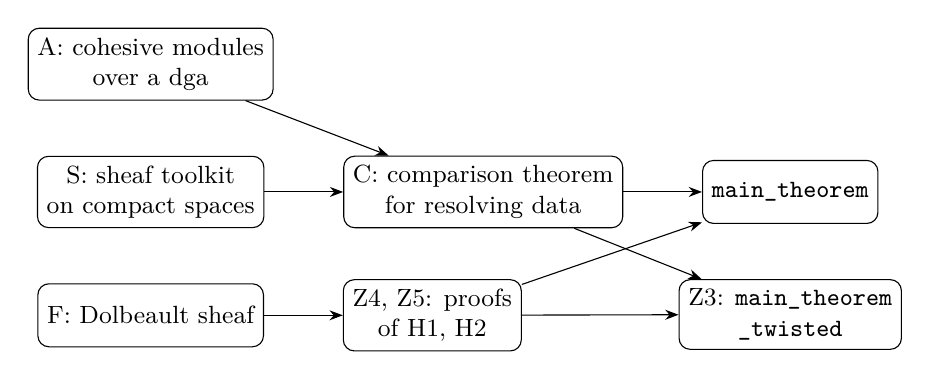
\begin{tikzpicture}[node distance=7mm and 10mm, box/.style={draw,rounded corners,align=center,font=\small,minimum height=8mm}]
\node[box] (A) {A: cohesive modules\\over a dga};
\node[box,below=of A] (S) {S: sheaf toolkit\\on compact spaces};
\node[box,below=of S] (F) {F: Dolbeault sheaf};
\node[box,right=of S] (C) {C: comparison theorem\\for resolving data};
\node[box,right=of F] (H) {Z4, Z5: proofs\\of H1, H2};
\node[box,right=of C] (M) {\code{main\_theorem}};
\node[box,below=of M] (T) {Z3: \code{main\_theorem}\\\code{\_twisted}};
\draw[-Stealth] (A) -- (C); \draw[-Stealth] (S) -- (C); \draw[-Stealth] (C) -- (M);
\draw[-Stealth] (F) -- (H); \draw[-Stealth] (H) -- (M);
\draw[-Stealth] (C) -- (T); \draw[-Stealth] (H) -- (T);
\end{tikzpicture}
\end{center}
The last step is short. F14 assembles resolving data from the Dolbeault data plus H1, H2:
\begin{lean}
def dolbeaultData (h₁ : DolbeaultGrothendieck E X) (h₂ : LocalGaugeLemma E X) : ResolvingData X :=
  { dolbeaultPreData E X with
    ρ_injective := dolbeaultRhoU_injective E
    exact0 := fun _ a ha ↦ exists_dolbeaultRhoU_of_dbar_eq_zero E a ha   -- F8: Cauchy–Riemann
    exactq := h₁
    LL := h₂ }

theorem blockPerf ... (h₁ : DolbeaultGrothendieck E X) (h₂ : LocalGaugeLemma E X) :
    (blockFunctor E X).Full ∧ (blockFunctor E X).Faithful ∧
      (blockFunctor E X).essImage = Perf (ringOf (holSheaf E X)) :=
  @ResolvingData.comparison _ _ (dolbeaultData E X h₁ h₂) _ _ h

theorem main_theorem : MainStatement := by
  intro E _ _ _ X _ _ _ _ _
  exact main_theorem_conditional E X (dolbeaultGrothendieck E X) (localGaugeLemma E X)
\end{lean}
Note that \code{exactq} and \code{LL} \emph{are} H1 and H2, verbatim. Most of the work is in the
abstract comparison theorem C6, \code{ResolvingData.comparison}: for resolving data on a compact
Hausdorff space, $J$ is full (C4), faithful (C4) and has essential image $\Dperf$ (C2 and C5). The
analytic work is in the proofs of H1 and H2 (\S\ref{sec:h1}, \S\ref{sec:h2}).

\subsection{Layer A: algebra of cohesive modules}
\begin{itemize}
\item \textbf{Connections} (A2): every finitely generated projective $A^0$-module has a
connection, via a splitting $P\oplus P'\cong(A^0)^m$.
\item \textbf{Form-degree filtration} (A6, A7): $\Hom^\bullet$ and total modules are finitely
filtered by form degree $b\in[0,N]$, $\mathrm{gr}^b\Hom\cong\Hom_{A^0}(Q_1,A^b\otimes Q_2)$. A map of
finitely filtered complexes inducing quasi-isomorphisms on all $\mathrm{gr}^b$ is a
quasi-isomorphism (proved by induction with the long exact sequence; this replaces the spectral
sequences of \cite{B} and \cite{A}).
\item \textbf{Lifting theorem} (A11) \cite[Thm~3.2.7]{B}, \cite[Prop~3.3.4]{A}: if each $A^b$ is flat over
$A^0$, $N$ is quasi-cohesive, $P$ a bounded complex of finitely generated projectives and
$e^0\colon P\to(Q_N,\X^0)$ a quasi-isomorphism, then $A\otimes P$ carries a cohesive structure
$\mathbb E$ with $\mathbb E^0=\partial_P$ and a closed degree-0 map $e\colon A\otimes P\to N$ extending
$e^0$. Proof: induction on form degree; at each step the defect is a cycle in an acyclic cone,
and a preimage gives the next components. All signs of \cite{A} were re-derived in the left
convention. The theorem holds for any curvature, which the twisted theorem uses.
\item \textbf{Total quasi-isomorphism} (A12): such $e$ is a quasi-isomorphism of total
complexes (A7 with the form-degree filtration).
\item \textbf{Adjunction} (A10.a): $\Hom^\bullet_{\mathcal P_A}(A\otimes_RW,M)\cong\Hom^\bullet_R(W,M)$.
\end{itemize}

\subsection{Layer S: sheaves on a compact space, without sheaf cohomology}
The sources use sheaf cohomology, softness on paracompact spaces, finite covering dimension and
Malgrange's flatness theorem. The formalization replaces all of them by elementary statements
that use compactness and fineness.
\begin{itemize}
\item \textbf{Fine rings} (S1--S3): over a fine sheaf of rings $S$, $\Gamma$ is exact on
$S$-modules (lift locally, glue with a partition of unity), so acyclic complexes of $S$-modules
have acyclic global sections.
\item \textbf{Soft sheaves} (S3.b): a sheaf of abelian groups on which $\Gamma(S)$ acts (additively,
unitally, locally) is soft, in a stalk-free form; a bounded-below acyclic complex with soft terms
has acyclic global sections. This is needed in C4, where the differentials are \emph{not}
$\cA^0$-linear.
\item \textbf{Projective modules} (S4): finite free $S$-modules are projective; locally free modules
of finite rank are summands of finite free ones; $\Gamma$ is an equivalence between such summands
and finitely generated projective $S(X)$-modules, with $\Hom_S(\tilde P,N)=\Hom_{S(X)}(P,N(X))$;
$\Gamma(\tilde P\otimes N)=P\otimes\Gamma(N)$.
\item \textbf{Locality, Hom sheaves} (S5--S7): restriction to opens, quasi-isomorphisms are local;
the Hom sheaf $\mathcal Hom(M,N)$, built on Mathlib's type-valued \code{presheafHom};
$\mathcal Hom(W,-)$ preserves quasi-isomorphisms for $W$ strictly perfect; $\mathcal Hom(C,I)$ is
acyclic for $C$ acyclic and $I$ a bounded-below complex of injectives.
\item \textbf{K-flat resolutions} (S8): every bounded-above complex has a K-flat resolution by
flat modules; K-flat acyclic $\otimes$ anything is acyclic; base change preserves
quasi-isomorphisms between K-flat complexes. \emph{This package replaces Malgrange's theorem}
($\cA$ flat over $\Ocal$), which \cite{A} assumes.
\item \textbf{Perfect complexes} (S9, S10): on compact $X$ a perfect complex is globally bounded;
over a fine $S$ every globally bounded perfect complex is quasi-isomorphic to a strictly perfect
one. The proof builds a finite free model by downward induction on degree, using local
null-homotopies, local lifting and local splitting, in place of \cite[Lemma~7.2.10]{A} on small opens
(which needs free modules over non-fine restrictions to be projective).
\item \textbf{Derived categories} (S11): wiring of Mathlib's injective resolutions,
K-injective and K-projective complexes.
\end{itemize}

\subsection{\texorpdfstring{An explicit model of $\cA\otimes_R K$ (C7)}{An explicit model of A ⊗ K (C7)}}
Sections of a sheafified tensor product are not computable, but several steps need them. For a
complex $K$ of $R|_U$-modules put $F:=\cA^0\otimes_R K$ and
\[ T(K)^n(V) := \Bigl(\cA(V)\otimes_{\cA^0(V)}\textstyle\bigoplus_p F^p(V)\Bigr)^n
= \textstyle\bigoplus_q \cA^q(V)\otimes_{\cA^0(V)} F^{n-q}(V), \]
with plain tensor products of sections.
\begin{itemize}
\item[C7.a] $T(K)^n$ is a sheaf: $\cA^q$ is a summand of a finite free $\cA^0$-module, so $T(K)^n$ is
sectionwise a retract of a finite power of $\bigoplus F$.
\item[C7.b,c] A flat connection $\nabla$ on $F$ (sheafify $\alpha\otimes k\mapsto d\alpha\otimes k$) gives
$\X(a\otimes f)=da\otimes f+(-1)^{|a|}(a\nabla f+a\otimes d_Ff)$; each $T(K)(V)$ is a quasi-cohesive
module over $\cA(V)$, and $T(K)$ is a complex of sheaves.
\item[C7.d] $T(K)\cong\cA^\bullet|_U\otimes K$ (Mathlib's tensor product of complexes, with the Koszul
sign on the first factor), and for $K$ bounded above with flat terms, $K\to T(K)$,
$k\mapsto1\otimes k$, is a quasi-isomorphism ($\rho$ is a resolution).
\item[C7.e,f] For $M$ cohesive over $\cA(U)$ and a closed degree-0 map $e$ into the global
sections of $T(K)$, the extension $\Xi_e\colon\alpha_U(M)\to T(K)$ is a chain map; it is a
quasi-isomorphism as soon as its form-degree-0 graded piece is one (filter both sides; $\mathrm{gr}^b$ is
a retract of a finite power of $\mathrm{gr}^0$).
\end{itemize}

\subsection{\texorpdfstring{$J$ lands in perfect complexes (C2)}{J lands in perfect complexes (C2)}}
Let $M$ be cohesive and $x\in X$. By H2 (field \code{LL}) there are $U'\ni x$, a bounded complex
$W$ of finitely generated projective $\Ocal(U')$-modules and a homotopy equivalence
$h\colon\cA(U')\otimes W\to M|_{U'}$. Let $\tilde W$ be the strictly perfect complex on $U'$ with
$\Gamma(\tilde W)=W$ (S4.c on the over-site). The map
$u\colon\tilde W\to\alpha_{U'}(\cA(U')\otimes W)$ is a quasi-isomorphism: compose with the
model $T(\tilde W)$, where $\Xi_e$ is a quasi-isomorphism by C7.f and $\tilde W\to T(\tilde W)$ one by
C7.d; conclude by 2-out-of-3. Then
\[ \alpha(M)|_{U'} \xleftarrow{\ \alpha(h)\circ u\ } \tilde W \xrightarrow{\ \mathrm{id}\ } \tilde W \]
is the roof required by \code{IsPerfect} (using $\alpha(M)|_{U'}\cong\alpha_{U'}(M|_{U'})$, C1.c).

\subsection{Full faithfulness (C4)}
For cohesive $M_1,M_2$ let $\mathcal H(M_1,M_2)(V)=\Hom^\bullet_{\mathcal P_{\cA(V)}}(M_1|_V,M_2|_V)$ (C3),
a complex of sheaves with $\Gamma(\mathcal H)=\Hom^\bullet_{\mathcal P_A}(M_1,M_2)$.
\begin{enumerate}
\item Choose a bounded-below injective resolution $r\colon\alpha(M_2)\to I$.
\item $\Psi\colon\mathcal H(M_1,M_2)\to\mathcal Hom(\alpha(M_1),I)$, $\varphi\mapsto r\circ\alpha(\varphi)$, is a map of
complexes of sheaves. $\Gamma(\cA^0)$ acts on the terms of both sides, so they are soft (S3.b),
although the differentials are not $\cA^0$-linear.
\item $\Psi$ is a quasi-isomorphism, checked locally. Near $x$ use $h$ and $u$ from C2:
\[\begin{tikzcd}[column sep=large,row sep=small]
\mathcal H(M_1,M_2)|_{U'} \arrow[r,"\Psi"] \arrow[d,"h^*"'] & \mathcal Hom(\alpha(M_1),I)|_{U'} \arrow[d,"\alpha(h)^*"]\\
\mathcal H(\cA\otimes W,M_2) \arrow[r,"\Psi"] \arrow[d,"\cong\ (\text{A10.a})"'] & \mathcal Hom(\cA\otimes_R\tilde W,I) \arrow[d,"u^*"]\\
\mathcal Hom(\tilde W,\alpha(M_2)) \arrow[r,"r_*"] & \mathcal Hom(\tilde W,I)
\end{tikzcd}\]
The upper vertical maps are sectionwise homotopy equivalences; $u^*$ is a quasi-isomorphism
because $\mathcal Hom(\mathrm{cone}(u),I)$ is acyclic (S7.c), and $r_*$ because $\tilde W$ is strictly perfect
(S7.b).
\item Hence $\Gamma(\Psi)$ is a quasi-isomorphism: its cone is bounded below, acyclic, with soft terms
(S3.b(iv)).
\item On $H^0$:
$\Hom_{\Ho(\mathcal P_A)}(M_1,M_2)\cong H^0\Hom(\alpha M_1,I)\cong\Hom_{D}(\alpha M_1,\alpha M_2)$,
and the composite is $J$ on morphisms. So $J$ is bijective on Hom sets.
\end{enumerate}

\subsection{Essential surjectivity (C5)}
Let $K$ be perfect.
\begin{enumerate}
\item $K$ is globally bounded (compactness); replace it by a bounded complex and then by a K-flat
resolution $K'\to K$ (S8).
\item $\cA^0\otimes_RK'$ is a globally bounded perfect complex of $\cA^0$-modules (S8).
\item Since $\cA^0$ is fine, it is quasi-isomorphic to a strictly perfect $\tilde P$ (S10), which is
K-projective, so there is an honest quasi-isomorphism $f^0\colon\tilde P\to\cA^0\otimes_RK'$.
\item Global sections: $P=\Gamma(\tilde P)$ is a bounded complex of finitely generated projective
$A^0$-modules and $\Gamma(f^0)$ a quasi-isomorphism (S3). $N:=\Gamma(T(K'))$ is quasi-cohesive (C7.c), and
each $A^q$ is flat over $A^0$, so the lifting theorem A11 gives a cohesive $M$ on $A\otimes P$ and
a closed $e\colon M\to N$ extending $\Gamma(f^0)$.
\item $\Xi_e\colon\alpha(M)\to T(K')$ is a quasi-isomorphism (C7.f: its $\mathrm{gr}^0$ is $f^0$).
\item $K'\to T(K')\cong\cA\otimes_RK'$ is a quasi-isomorphism (C7.d: $\rho$ is a resolution, $K'$ is K-flat).
\item Hence $J(M)=\alpha(M)\cong T(K')\cong K'\cong K$ in $D(\Ocal)$.
\end{enumerate}
Conversely every $J(M)$ is perfect by C2, so the essential image is exactly $\Dperf$. This is C6.

\subsection{Proof of H1: the Dolbeault--Grothendieck lemma (Z4)}\label{sec:h1}
\code{dolbeaultGrothendieck : DolbeaultGrothendieck E X} holds on every complex manifold modelled
on a finite-dimensional $E$, without compactness \cite[Thm~2.3.3]{Hor}, \cite[p.~25]{GH}.
\begin{itemize}
\item \textbf{One variable} (Z4.a--b): $t\mapsto t^{-1}$ is locally integrable on $\mathbb C$, and the
Cauchy transform $u(w)=\pi^{-1}\int t^{-1}h(w-t)\,dA(t)$ solves $\partial u/\partial\bar w=h$ for
compactly supported $C^1$ $h$ with values in a complex Banach space (Cauchy--Pompeiu; a port of
the TauCeti file \code{Pompeiu.lean} \cite{TauCeti}, Apache~2.0).
\item \textbf{With parameters} (Z4.c): the solver
$\mathrm{cauchySolve}\,v\,F(z)=\pi^{-1}\int t^{-1}F(z-tv)\,dA(t)$ along the complex lines $z+\mathbb Cv$,
$v\ne0$, is $C^\infty$ when $F$ is, commutes with derivatives and with continuous
$\mathbb C$-linear maps, and is a right inverse of $\dbar$ along $v$.
\item \textbf{Several variables} (Z4.d--e): induction on the number of basis directions
$d\bar z_0,\dots,d\bar z_k$ that the closed form $\beta$ involves. The step contracts $\beta$ with
the $k$-th basis vector, cuts the result off (a cutoff constant in the other directions, on a slab
stable under translation along $e_k$), solves along $e_k$, and subtracts $\dbar$ of the solution;
the cutoff is applied before solving, so all statements are global on $E$. This gives the flat
lemma \code{exists\_dbar\_eq} on open subsets of $E$, with a primitive smooth on all of $E$.
\item \textbf{On $X$} (Z4.f--g): write the form in the chart at $x$, solve there, and carry the
primitive back as a Dolbeault form (\code{chartForm}); no general chart transport (F13) is needed.
\end{itemize}

\subsection{Proof of H2: the local gauge lemma (Z5)}\label{sec:h2}
\code{localGaugeLemma : LocalGaugeLemma E X} holds on every complex manifold, without compactness
(\cite[proof of Lemma~4.1.5]{B}; \cite[\S2.2.2]{DK}; \cite[Thm~5.3]{BSW}).
\begin{itemize}
\item \textbf{Frames} (Z5.g--h): near $x$ the base-changed generators
$\cA^0(U')\otimes_{\cA^0(X)}Q^p$ are free (by localization at the maximal ideal of $x$, not by
idempotent matrices). In a chart and a graded frame, $\X=\dbar+\mathcal A$ with $\mathcal A$ a
smooth function with values in odd fibre operators on $\Lambda^{0,\bullet}\otimes\mathbb C^r$, and
flatness is the Maurer--Cartan equation $\sum_j\varepsilon_j\partial_j\mathcal A+\mathcal A^2=0$
($\varepsilon_j=d\bar z_j\wedge\cdot$).
\item \textbf{Gauge induction} (Z5.e--f): a gauge $g$ (even, of degree $0$, smooth, invertible)
acts by $g\cdot\mathcal A=g\mathcal Ag^{-1}-(\sum_j\varepsilon_j\partial_jg)g^{-1}$. One coordinate at a
time, a gauge removes the $d\bar z_k$-coefficient $a_k=\iota_k\mathcal A+\mathcal A\iota_k$; once
all $a_i$ vanish, the contracted Maurer--Cartan equation gives $\partial_i\mathcal A=0$, so the
remaining operator is holomorphic of form degree $0$.
\item \textbf{The step} (Z5.a--c): solve the \emph{linear} equation $\dbar_kg=ga$ with parameters by
a Neumann series $g=\sum_iu_i$ of iterated Cauchy solves. The kernel estimate
$\|\mathrm{cauchySolve}\,v\,G\|\le3\rho\sup\|G\|$ on slabs of width $\rho$ makes the series converge
with all derivatives (summable bounds $\|D^mu_i\|\le C_m(i+1)^m\theta^i$, $\theta<1$), so $g$ is
$C^\infty$ without elliptic regularity; the constraints on $g$ are kept by solving in a subalgebra.
\item \textbf{Assembly} (Z5.i): the holomorphic degree-$0$ entries are $\rho(f_{ij})$ with
$f_{ij}\in\Ocal(U'')$ (F12); $W$ is the free complex of the matrix $f$, and the gauge matrices
$G,H$ give mutually inverse closed maps $M|_{U''}\rightleftarrows\cA(U'')\otimes W$.
\end{itemize}
The proof establishes the strong form (an isomorphism of cohesive modules, $W$ free) in substance,
and concludes the weak form H2. It does not use H1, only the analytic toolkit of Z4.

\subsection{The twisted theorem (Z3)}\label{sec:tw-proof}
Twisted sheaves have no global sections, so every global step (softness, globalization, lifting)
acts on untwisted objects, and every local step is the flat theory above on $U_\alpha$ after the
gauge $\X\mapsto\X-h^0_\alpha$.
\begin{itemize}
\item \textbf{Gauge} (Z3.b): for $c'=c+d\beta$, $M\mapsto(Q,\X-\beta\cdot)$ identifies
$\Ho(\mathcal P_{(\cA,c')})$ with $\Ho(\mathcal P_{(\cA,c)})$; the Hom complexes agree on the nose.
\item \textbf{Twist data} (Z3.d): every closed $h$ has one, built from local primitives given by H1
in degrees $2$ and $1$ and exponentials; no Leray cover is needed.
\item \textbf{Twisted sheaves} (Z3.f--l, r): the abelian category \code{TwMod} with enough
injectives (Toda's twisted pushforward \cite[Lemma~4.3]{Toda}), gluing $\mathrm{TwMod}(U,1)\simeq\mathrm{Mod}$, rescaling,
extension by zero, base change and twisted Hom sheaves.
\item \textbf{Locally flat} (Z3.o): $J_T(M)_\alpha\cong\alpha_{U_\alpha}(\mathrm{gauge}_{h^0_\alpha}(M|_{U_\alpha}))$,
which reduces perfection (Z3.p) and the local step of full faithfulness (Z3.s) to C2 and C4 on
$U_\alpha$, with H2 over opens (Z3.e).
\item \textbf{Essential surjectivity} (Z3.t--u): base-change a flat local model to $\cA^0$, untwist it
by $u^{-1}$ and glue it to a perfect complex of $\cA^0$-modules on $X$, glue the local connections
plus $h^0_\alpha$ to a curved connection, and lift by A11 (which holds for any curvature).
\end{itemize}
The C1/C3/C7 constructions assume $c=0$; Z3 copies the needed terms over \code{DgaSheafData}, the
version of the resolving data without the field $c=0$.

\subsection{\texorpdfstring{The triangulated structure and K4 (Z2)}{The triangulated structure and K4 (Z2)}}\label{sec:tr}
Not used by the statements, but proved: \code{instance : IsTriangulated (HoP 𝒜)} for every
bounded graded-commutative curved dga (\cite[Prop~2.4.1]{B}, whose proof refers to \cite[Props~1--2]{BK}).
Shifts are transported along a sign isomorphism $\iota_a$ (Block's $\mathbb E[1]=-\mathbb E$ is
correct only for right modules), cones have generators $Q_N^p\times Q_M^{p+1}$, and every formula
matches Mathlib's \code{HomotopyCategory} conventions (shift, mapping cone, third map
$-\iota_1^{-1}\circ\mathrm{fst}$); the proofs follow Mathlib's \code{HomotopyCategory} files step
by step. Check K4: $(\cA\to\cA[n])\cong H^{0,n}_{\dbar}(X)$ for the unit module, for every
$n\in\mathbb Z$, which confirms the shift. That $J$ is a triangulated functor is not formalized.

\subsection{\texorpdfstring{An independent check of $\dbar$ (K7)}{An independent check of dbar (K7)}}\label{sec:k7}
\code{ChecksK7.lean} transcribes TauCeti's $\bar\partial$ \cite{TauCeti} (type projections of the exterior
derivative for the complex structure $J=i\cdot$) on the model space $E$ and proves
(\code{tcDelBar\_toReal}) that it agrees with our $\dbar$ on $(0,q)$-forms read as real forms. The
transcription was checked in excerpts at gate~13.

%======================================================================
\section{Deviations from the sources}
\begin{enumerate}
\item $\Dperf$ instead of $D^b_{\mathrm{coh}}$ (\cite{B} states the theorem for $D^b_{\mathrm{coh}}$; the step
$\Dperf=D^b_{\mathrm{coh}}$ on compact complex manifolds needs Oka's coherence theorem and is not
formalized, Z1). The same for the twisted theorem.
\item The equivalence is stated as full, faithful, essential image $=\Dperf$; equivalent to the
corestriction form (K6, proved).
\item Left modules instead of Block's right modules; curvature $c\leftrightarrow-c$ ($c=h$ of \cite{A},
$-B$ of \cite[\S4.2]{B}); no factor $2\pi i$.
\item Finite covers and compactness replace softness on paracompact spaces and finite covering
dimension; elementary acyclicity statements (S3, S3.b) replace sheaf cohomology.
\item K-flat resolutions replace Malgrange's flatness theorem (\cite{A}'s Assumption~5, first half).
\item H2 is the weak form: an isomorphism in $\Ho(\mathcal P)$ rather than of cohesive modules, $W$
projective rather than free, stated on sections over small opens and only for restrictions of
global cohesive modules. H1 and H2 are stated on $X$, not on open subsets of $E$. Their proofs
work for any finite-dimensional $E$ (no coordinates $\mathbb C^n$, no polydiscs).
\item In the proof of H2, the kernel bound is $3\pi\rho$ instead of \cite{DK}'s $2\pi\rho$ (the disc is
not centred at the pole); local freeness by localization; the smoothness of the gauge is proved
by summable derivative bounds, which closes a gap in the sources.
\item $(0,q)$-forms are $\mathbb C$-alternating maps on $\bar E$; the product is transported from the
exterior algebra of the antilinear dual.
\item $\alpha(M)^n(V)$ is spelled through the base change $M|_V$, canonically isomorphic to Block's
$\bigoplus_{p+q=n}\cA^q(V)\otimes Q^p$.
\item Twisted theorem: stated for every twist datum $T$ (finite cover, normalized $\hc$,
multiplicative data $(h^0,u,\hc)$ instead of \cite{A}'s $(h^0,h^1,h^2,\exp_{\mathcal R})$); independence
of $T$ is not formalized. Twisted sheaves glue by maps on sections over every open, with
$\varphi_{\alpha\alpha}=\mathrm{id}$ as an axiom (\cite{A} only gets $\varphi_{\alpha\alpha}$ idempotent, and
$\varphi=0$ would satisfy the other axioms); $\mathrm{TwPerf}$ is componentwise; no intermediate
category of cdg-modules.
\item Errata found in the sources: in \cite{A}, ``Assumption 7'' means item~6, item~6's target is
$A^*\otimes_RW$, Prop.~7.2.18 forms $A^0\otimes_RM$ underived (fixed by 5), and the cocycle
condition of Def.~7.1.1, $\varphi_{\alpha\beta}\circ\varphi_{\beta\gamma}=\hc\varphi_{\alpha\gamma}$, does
not typecheck (we use $\varphi_{\beta\gamma}\circ\varphi_{\alpha\beta}=\hc_{\alpha\beta\gamma}\varphi_{\alpha\gamma}$);
in \cite[proof of Lemma~3.2.8]{B} two typos; \cite{A}'s signs re-derived in the left convention.
\end{enumerate}

%======================================================================
\section{What to trust, and how it was checked}
\begin{itemize}
\item \textbf{Trusted base.} The Lean kernel, Mathlib \code{v4.35.0}, and the 44 frozen files that
the three statements depend on (276 declarations, listed with docstrings in
\code{review/statement-defs.md}). Everything else is proof and is checked by the kernel.
\item \textbf{No axioms beyond Lean's}: \code{\#print axioms} for \code{main\_theorem},
\code{main\_theorem\_conditional} and \code{main\_theorem\_twisted} gives
\code{[propext, Classical.choice, Quot.sound]} (checked automatically by \code{\#guard\_msgs} in
\code{ChecksMain.lean} and \code{ChecksTwistedMain.lean}); no \code{sorry}, \code{admit},
\code{native\_decide}, \code{unsafe} or custom \code{axiom} in the project.
\item \textbf{Human review in gates.} The work proceeded in phases (algebra, local analysis,
sheaf toolkit, Dolbeault sheaf, comparison, assembly; then the proofs of H1 and H2, the twisted
theorem, the triangulated structure). At each of 14 gates the new definitions and statements
were presented to a human on a generated review sheet and checked in excerpts, and the
definitions entering the statements were frozen (a hook refuses edits to frozen files).
\item \textbf{Non-vacuity.} Every definition has a satisfiable example; H1 and H2 are proved
directly in dimension $0$; every closed $h$ has a twist datum; normalizations such as
$\dbar\bar z=d\bar z$ and $\dbar|z|^2=z\,d\bar z$ on $\mathbb C$ are proved; K4 computes Dolbeault
cohomology as Hom sets in $\Ho(\mathcal P_A)$; K7 compares $\dbar$ with an independent definition;
K8 derives the untwisted statement from the twisted one; a curved toy dga has cohesive modules
(K12).
\item \textbf{Size.} About 300 Lean files and 72\,000 lines (without the documentation hubs),
written between 21 October and 8 November 2026.
\item \textbf{Not formalized} (deferred on purpose): $\Dperf=D^b_{\mathrm{coh}}$ (Z1); independence of
the twist datum; $J$ and $J_T$ as triangulated functors; open (non-compact) manifolds; the full
chart transport of Dolbeault forms (F13).
\end{itemize}

%======================================================================
\begin{thebibliography}{TauCeti}
\bibitem[A]{A} P.~Antweiler, \emph{Curved $\infty$-local systems and projectively flat
Riemann--Hilbert correspondence}, arXiv:2411.19595v1, 2024.

\bibitem[B]{B} J.~Block, \emph{Duality and equivalence of module categories in noncommutative
geometry}, in: A celebration of the mathematical legacy of Raoul Bott, CRM Proc.\ Lecture
Notes~50, Amer.\ Math.\ Soc., 2010; arXiv:math/0509284v2 (numbering of the arXiv version).

\bibitem[BK]{BK} A.~Bondal, M.~Kapranov, \emph{Enhanced triangulated categories}, Math.\ USSR
Sb.~70 (1991), 93--107.

\bibitem[BSW]{BSW} J.-M.~Bismut, S.~Shen, Z.~Wei, \emph{Coherent sheaves, superconnections, and
Riemann--Roch--Grothendieck}, Progr.\ Math.~347, Birkhäuser, 2023; arXiv:2102.08129.

\bibitem[Că]{Cal} A.~Căldăraru, \emph{Derived categories of twisted sheaves on Calabi--Yau
manifolds}, PhD thesis, Cornell University, 2000.

\bibitem[CHL]{CHL} J.~Chuang, J.~Holstein, A.~Lazarev, \emph{Maurer--Cartan moduli and theorems
of Riemann--Hilbert type}, Appl.\ Categ.\ Structures~29 (2021); arXiv:1802.02549v3 (numbering of
the arXiv version).

\bibitem[DK]{DK} S.~K.~Donaldson, P.~B.~Kronheimer, \emph{The geometry of four-manifolds}, Oxford
University Press, 1990.

\bibitem[GH]{GH} P.~Griffiths, J.~Harris, \emph{Principles of algebraic geometry}, Wiley, 1978.

\bibitem[Hö]{Hor} L.~Hörmander, \emph{An introduction to complex analysis in several variables},
3rd ed., North-Holland, 1990.

\bibitem[Mathlib]{Mathlib} The mathlib Community, \emph{The Lean mathematical library}, in: Proc.\
CPP 2020, ACM, 2020, 367--381; version \code{v4.35.0}.

\bibitem[TauCeti]{TauCeti} The TauCeti project, Lean formalization library,
\url{https://github.com/TauCetiProject/TauCeti} (branch \code{main}, fetched 1 November 2026;
Apache License~2.0).

\bibitem[Toda]{Toda} Y.~Toda, \emph{Deformations and Fourier--Mukai transforms}, J.\ Differential
Geom.~81 (2009), 197--224.
\end{thebibliography}

\end{document}
